\documentclass[10pt,a4paper,notitlepage, twocolumn]{article}
\usepackage[utf8]{inputenc}
\usepackage{amsmath}
\usepackage{amsfonts}
\usepackage{graphicx}
\usepackage{amssymb}
\usepackage{float}
\usepackage{listings}
\usepackage{lipsum}

\author{Nathaniel Forde}
\title{Decision and Expected Value}
\begin{document}


\section*{The Workhorse}

There is an unsung hero in data-science today. An algorithm  both ubiquitous and under appreciated. It's pivotal for nearly every project and informs the actions of tech giants and policy makers the world over. It is only mildly hyperbolic to say that understanding this formula unlocks wealth and power. It lies at the heart of online A/B testing, all policy analysis, sound business strategy and poker play.
$$ EV(O)_{p} = p_{1}v(o_{1}) + p_{2}v(o_{2}) + ... + p_{k}v(o_{k}) $$
In words: The expected financial value of a repeated process resulting in set of mutually exclusive outcomes is just the sum of their respective value weighted by the probability of each outcome. Outcomes can vary from deals of cards, to customer journeys and elections. \footnote{In the jargon $O$ is a random variable which can be realised as any of the outcomes  $ o_{j} :  1 \leq j \leq k$} 
But aside from the mercenary possibilities, the formula merits your attention for the light it sheds on the puzzling topic of probabilities. With stakes on the line the meaning of probability is no idle concern.

\subsubsection*{Two sides of a Coin}
Probability has a dual aspect. On one reading it refers to the long run tendency of a random process, on another the probability is construed as the degree of belief in the an outcome. On the first interpretation the probability is a distribution with certain fixed characteristics (e.g. a uniform probability distribution is assumed in the roll of die, where all outcomes are equally likely). On the second reading the characteristics of the probability distribution are learned from the data. These approaches are united by the Law of Large numbers which states that as the size of our sample increases our sample average will converge to the expected realisation of the process.
$$  \frac{1}{N} \sum_{i = 1}^{N} O_{i} \text{ converges to }  E(O) \text{ as } N \text{ approaches } \infty $$ In the attached plot we have stipulated a Poisson distribution with a mean of 4.5 and see how three examples of how consecutive averaging from the increasing sample sizes results in a close convergence to the population mean.
\begin{figure}[H]
  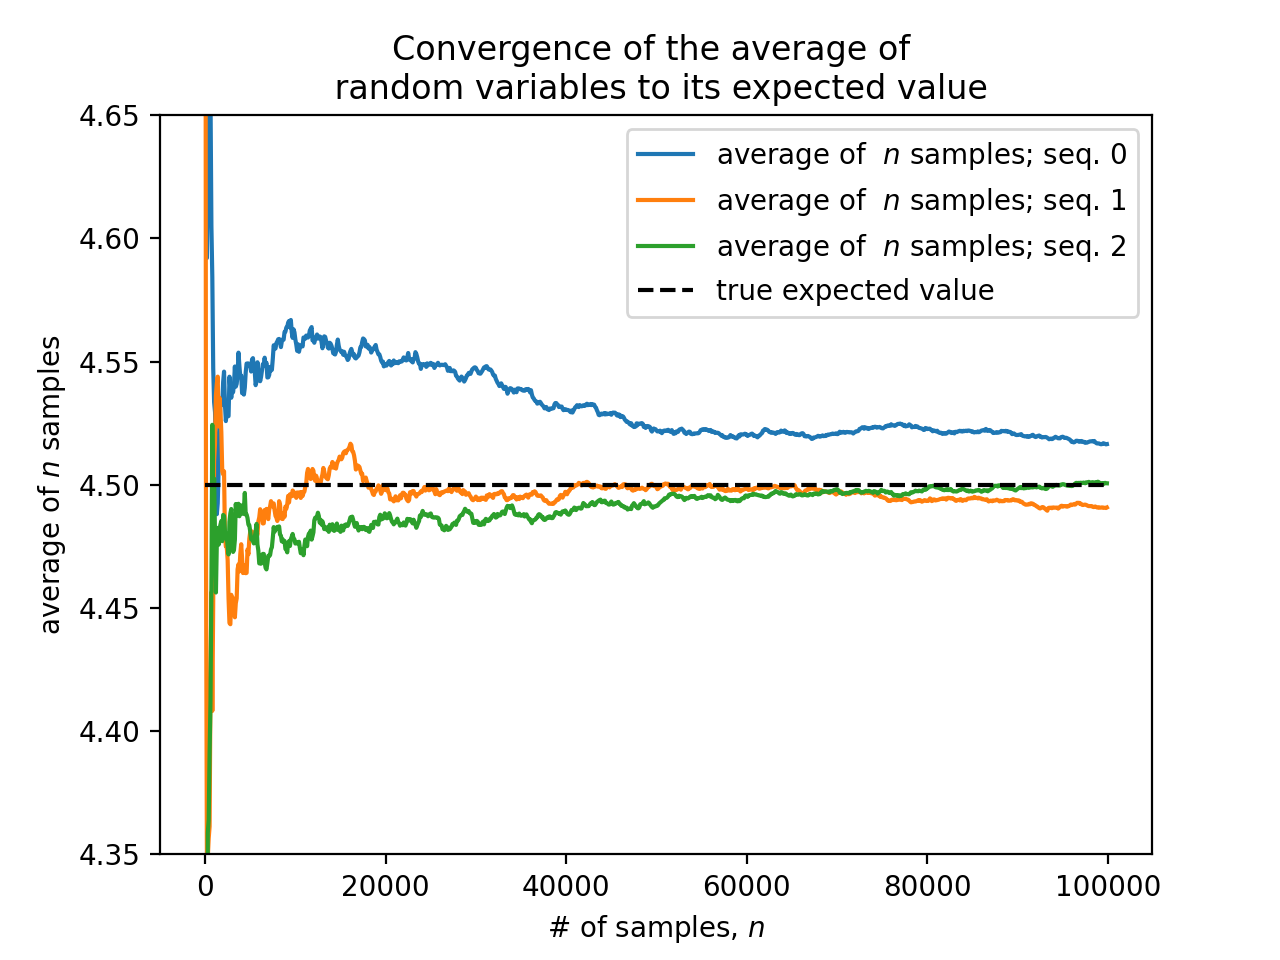
\includegraphics[width=\linewidth]{./Plots/convergence_of_law_of_large_numbers.png}
\end{figure}

\noindent This is fundamental to the long-run tendency interpretation of probability. Given a game with fixed and fair odds we see that repeated play will converge because of characteristics which govern the process. Dice are the paradigm example.  In the wild we never know the characteristics which cause the spread of outcomes, but such is the influence of gambling on the consideration of probability, that the default reading assumes a stability in the generating process. Partially this is pragmatic. The maths are more tractable if we can assume one well behaved underlying process. The results are compelling. The Normal (Bell Curve) distribution, the Poisson distribution the Bernoulli distribution (to name a few) are all rightly famous. Their shapes are characteristics of innumerable random processes. But the paradigm clouds the fact that in practice we start on the left side of the law of large numbers (with samples) and we often start with small numbers. 
\begin{figure}[H]
  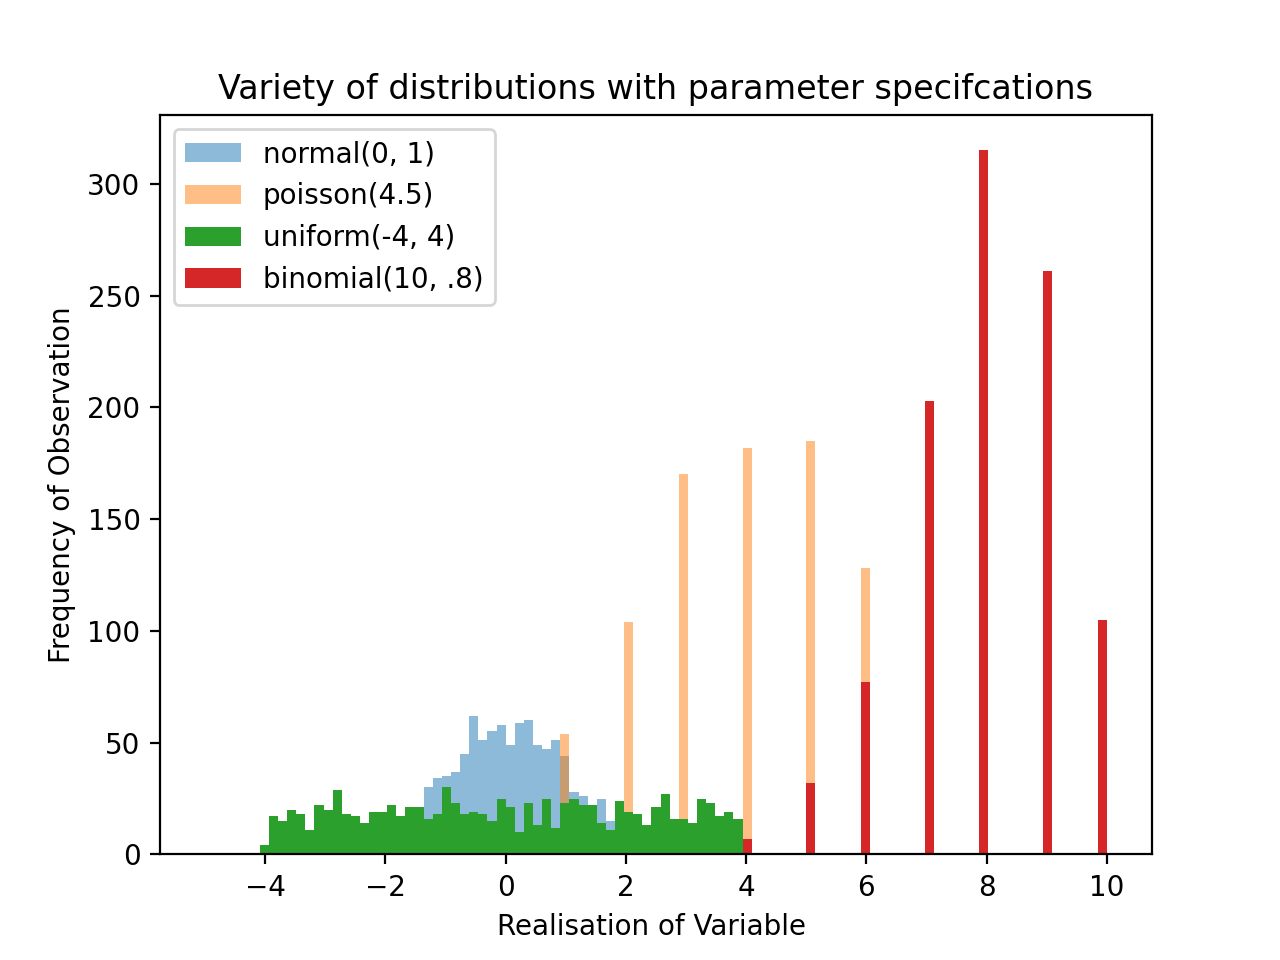
\includegraphics[width=\linewidth]{./Plots/variety_of_distributions.png}
\end{figure}
Well behaved probability distributions are rare beasts; a tiny fraction of the world's arbitrary menagerie. The fundamental question in probability is not whether probability is a measure of belief or frequency - it is whether we can safely assume that the underlying process adheres to a known model? If so, we can rely on the structure of the distribution to inform inference, if not we are better learning from the data - trusting to the sampling distribution and worst scenario planning.


\subsubsection*{Change points, Errors and Expectations}
When your only tool is a hammer, then everything is a nail. When one model won't do, use two. This is roughly the approach adopted when models fail. The problem is especially vivid in time-series forecasts; projected death rates, body counts and stock prices are all subject to sudden shocks. In the below graph we have a series characterised by change. After the first shock we can refit the model so that the line tracks well with the evolving data. After the second shock we try another refit, but the range the and variance of the data makes our basic model a poor fit. This presents three examples of uncertainty in the modelling process: (i) forecasts fail for the reason that's it's also difficult to identify (in the moment) those changepoints in the data which reflect structural change, (ii) the second linear model is a good fit and the fundamental assumptions that go into the model are sound, but the parameters need be re-estimated based on the new data
\begin{figure}[H]
  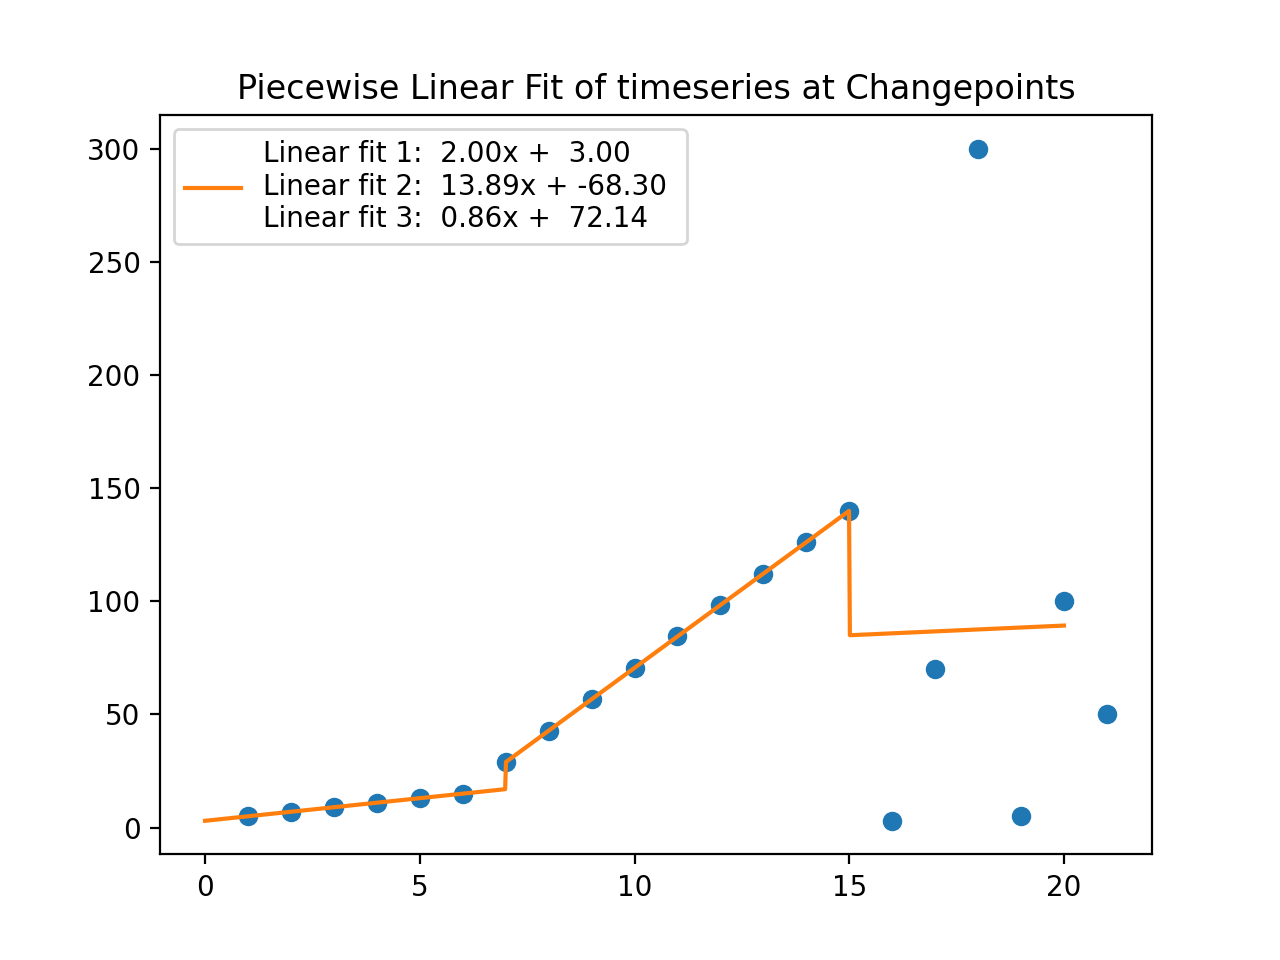
\includegraphics[width=\linewidth]{./Plots/piecewise_linear_fits.png}
\end{figure}
and (iii) the third linear model is simply a terrible fit for the data. In practice you never really know whether a new error stems from a misfit but appropriate model or an entirely inappropriate model. The piecewise linear fits makes use of the ordinary least squares technique to fit the slope of a line to each segment of the data. As we increase our number of sample fits we hope to better approximate the true linear function (if any) encoded in the data. This warrants a note about errors.

\noindent Imagine now that our previous graph showing three segments of data is extended infinitely in both directions.We can then slice this line into n-segments and refit a new model for each segment. If the underlying data generating process is stable we'd expect that on average the parameter fits converge to the characteristics of the stable process. Our sample estimates will overshoot in some cases and nearly miss in others, but on the whole the errors will cancel each other out.
\newline

The code example below builds two sampling distributions based on different underlying processes.  One in which the errors are independent, normally distributed around 0 the other in which the errors are correlated in sine-wave like pattern increasing and decreasing periodically. This is akin to difference between measuring error when predicting the heights of randomly sampled people versus predicting the sales volumes on randomly selected days of the week. A random sample of daily sales  risks clumping weekends together and skewing the expected values. No such risk exists when sampling from independent individuals. 

\begin{lstlisting}[language=Python]
### Build True Models
N = 100000
X = np.random.uniform(0, 20, N)
uncorrelated_errors = np.random.normal(0, 10, N)
correlated_errors = np.random.uniform (0, 10) + 
np.sin(np.linspace(0, 10*np.pi, N)) + 
np.sin(np.linspace(0, 5*np.pi, N))**2 + 
np.sin(np.linspace(1, 6*np.pi, N))**2

Y_corr = -2 + 3.5 * X + correlated_errors
Y = -2 + 3.5 * X + uncorrelated_errors
population = pd.DataFrame({'X': X, 'Y': Y, 
'Y_corr': Y_corr})

### Sample from Data and build smaller models
fits = pd.DataFrame(columns=['iid_const',
 'iid_beta', 'corr_const', 'corr_beta'])
for i in range(0, 10000):
    sample = population.sample(n=100, 
    replace=True)
    Y = sample['Y']; X = sample['X']
    Y_corr = sample['Y_corr']
    X = sm.add_constant(X)
    iid_model = sm.OLS(Y, X)
    results = iid_model.fit()
    corr_model = sm.OLS(Y_corr, X)
    results_2 = corr_model.fit()
    row = [results.params[0], 
    results.params[1],
    results_2.params[0], 
    results_2.params[1]]
    fits.loc[len(fits)] = row
    
fits.boxplot()
\end{lstlisting}


\begin{figure}[H]
  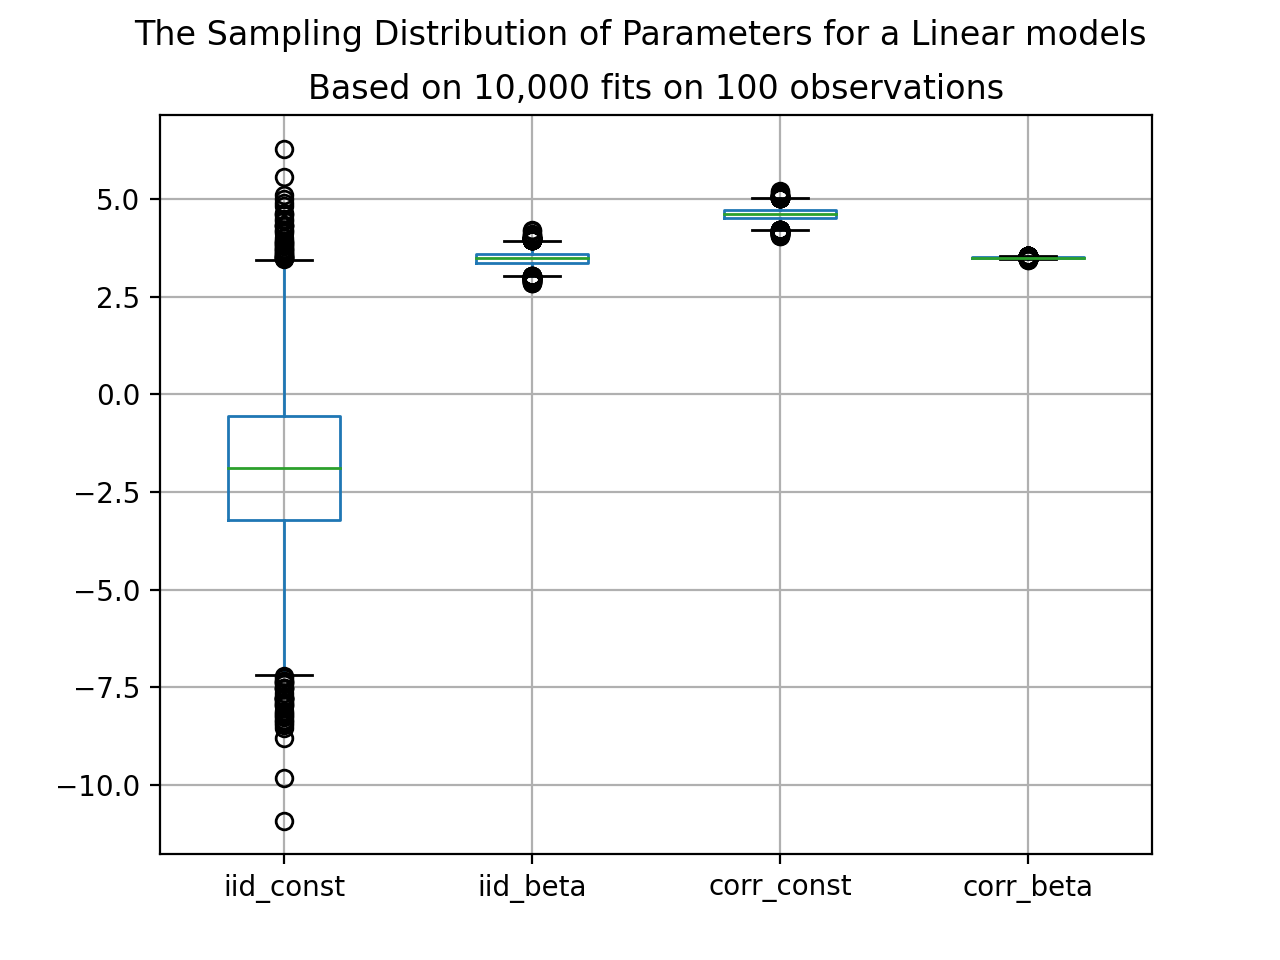
\includegraphics[width=\linewidth]{./Plots/distribution_of_beta1.png}
\end{figure}

In the first case the symmetry of the normal pattern ensures expected value for our parameter estimates match almost exactly the true values of the process. In the second model with correlated errors  the parameter estimate for our constant is 4.9 which is significantly different from the true value of -2, and will lead to systematically skewed predictions.

\subsubsection*{Small World of the Model}



\end{document}

